%% This is file `elsarticle-template-1a-num.tex',
%%
%% Copyright 2009 Elsevier Ltd
%%
%% This file is part of the ' Bundle'.
%% ---------------------------------------------
%%
%% It may be distributed under the conditions of the LaTeX Project Public
%% License, either version 1.2 of this license or (at your option) any
%% later version.  The latest version of this license is in
%%    http://www.latex-project.org/lppl.txt
%% and version 1.2 or later is part of all distributions of LaTeX
%% version 1999/12/01 or later.
%%
%% The list of all files belonging to the 'Elsarticle Bundle' is
%% given in the file `manifest.txt'.
%%
%% Template article for Elsevier's document class `elsarticle'
%% with numbered style bibliographic references
%%
%% $Id: elsarticle-template-1a-num.tex 151 2009-10-08 05:18:25Z rishi $
%% $URL: http://lenova.river-valley.com/svn/elsbst/trunk/elsarticle-template-1a-num.tex $
%%

\documentclass[preprint,12pt]{elsarticle}

%% Use the option review to obtain double line spacing
%%\documentclass[preprint,review,12pt]{elsarticle}

%% Use the options 1p,twocolumn; 3p; 3p,twocolumn; 5p; or 5p,twocolumn
%% for a journal layout:
 %%\documentclass[final,1p,times]{elsarticle}
%%\documentclass[final,1p,times,twocolumn]{elsarticle}
%% \documentclass[final,3p,times]{elsarticle}
%\documentclass[final,3p,times,twocolumn]{elsarticle}
%% \documentclass[final,5p,times]{elsarticle}
%%\documentclass[final,5p,times,twocolumn]{elsarticle}

%% if you use PostScript figures in your article
%% use the graphics package for simple commands
%% \usepackage{graphics}
%% or use the graphicx package for more complicated commands
 \usepackage{graphicx,psfrag}
%% or use the epsfig package if you prefer to use the old commands
%% \usepackage{epsfig}

%% The amssymb package provides various useful mathematical symbols
\usepackage{amssymb}
%% The amsthm package provides extended theorem environments
%% \usepackage{amsthm}

%% The lineno packages adds line numbers. Start line numbering with
%% \begin{linenumbers}, end it with \end{linenumbers}. Or switch it on
%% for the whole article with \linenumbers after \end{frontmatter}.
%% \usepackage{lineno}

%% natbib.sty is loaded by default. However, natbib options can be
%% provided with \biboptions{...} command. Following options are
%% valid:

%%   round  -  round parentheses are used (default)
%%   square -  square brackets are used   [option]
%%   curly  -  curly braces are used      {option}
%%   angle  -  angle brackets are used    <option>
%%   semicolon  -  multiple citations separated by semi-colon
%%   colon  - same as semicolon, an earlier confusion
%%   comma  -  separated by comma
%%   numbers-  selects numerical citations
%%   super  -  numerical citations as superscripts
%%   sort   -  sorts multiple citations according to order in ref. list
%%   sort&compress   -  like sort, but also compresses numerical citations
%%   compress - compresses without sorting
%%
%% \biboptions{comma,round}

% \biboptions{}

\begin{document}

%% Title, authors and addresses

%% use the tnoteref command within \title for footnotes;
%% use the tnotetext command for the associated footnote;
%% use the fnref command within \author or \address for footnotes;
%% use the fntext command for the associated footnote;
%% use the corref command within \author for corresponding author footnotes;
%% use the cortext command for the associated footnote;
%% use the ead command for the email address,
%% and the form \ead[url] for the home page:
%%
%% \title{Title\tnoteref{label1}}
%% \tnotetext[label1]{}
%% \author{Name\corref{cor1}\fnref{label2}}
%% \ead{email address}
%% \ead[url]{home page}
%% \fntext[label2]{}
%% \cortext[cor1]{}
%% \address{Address\fnref{label3}}
%% \fntext[label3]{}



%% use optional labels to link authors explicitly to addresses:
%% \author[label1,label2]{<author name>}
%% \address[label1]{<address>}
%% \address[label2]{<address>}
\newcommand{\plus}{\raisebox{.3\height}{\scalebox{.6}{+}}}
\newcommand{\minus}{\raisebox{0\height}{\scalebox{1}{-}}}
\section{Polarized Target} \label{Target}
\subsection{Description} \label{Description}
The proposed experiment will utilize a new, dynamically polarized target under construction for the CLAS12 spectrometer by a collaboration of the Jefferson Lab Target Group, the University of Virgina, Old Dominion University and Christopher Newport University.  The target cryostat, shown schematically in Figure~\ref{Target}, is specifically designed according to the geometrical constraints imposed by the CLAS12 detector package, primarily the Silicon Vertex Tracker.  Frozen, deuterated ammonia has been chosen as the target material for its high deuteron content (30\% by weight), high deuteron polarization (up to 50\%), and high resistance to radiation damage \cite{Goertz2002}.  Construction of the target is currently underway, with initial tests anticipated in 2017.

\begin{figure}
\begin{center}
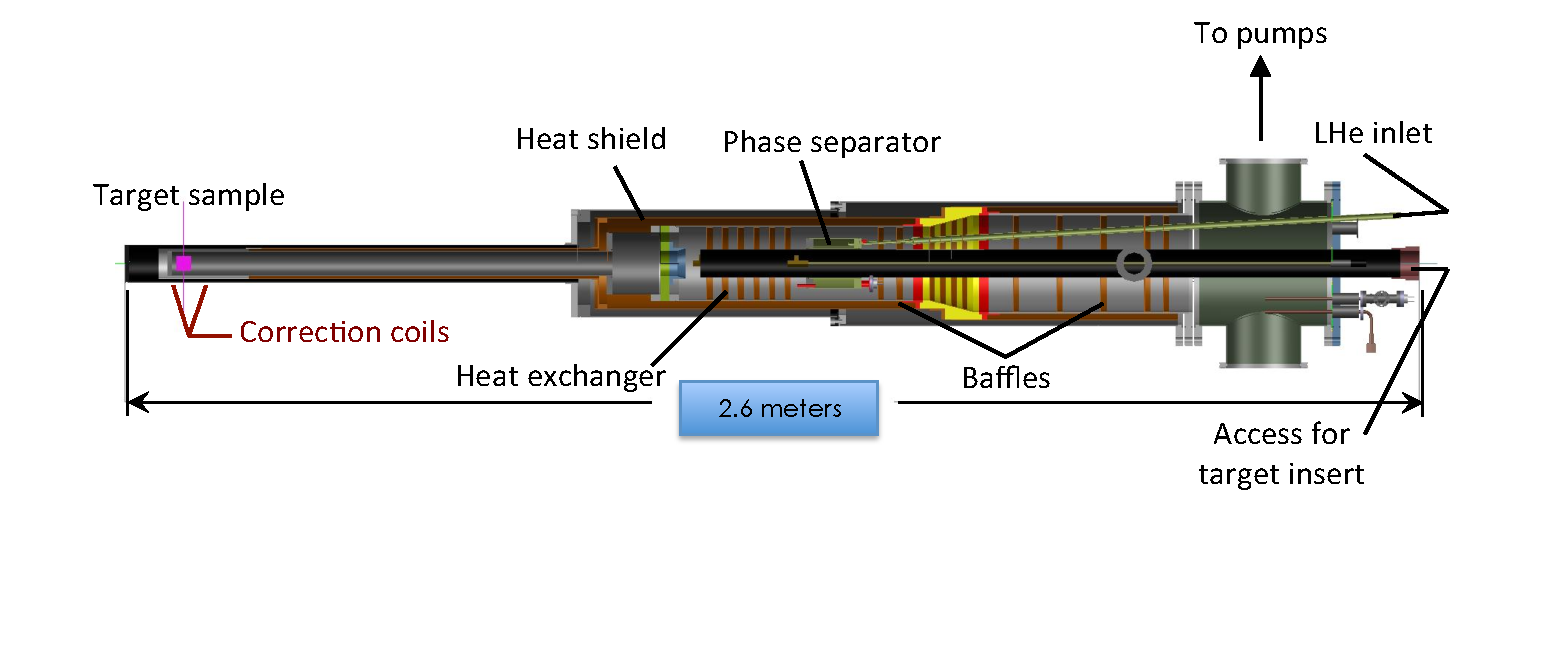
\includegraphics[width=5.5in]{Target_Side.pdf}
\end{center}
\caption{Side view of the CLAS12 dynamically polarized target.}
\label{Target}
\end{figure}

To realize Dynamic Nuclear Polarization (DNP), a dielectric solid is doped with a small concentration 
($10^{19}$~cm$^{\minus3}$) of paramagnetic radicals.  The unpaired electrons in the radicals are highly polarized by cooling the sample to a low temperature and applying a strong magnetic field.  For example, at the proposed operating conditions of 1~K and 5~T, the electron polarization is greater than 99.99\%.  Off-center microwave saturation of the electron spin resonance drives mutual electron/nuclear spin flips which effectively transfer the electron polarization to the nuclei.  Either positive or negative nuclear polarization can be realized, depending on whether the microwave frequency is slightly below or above the electron resonance frequency of 140~GHz.

The nominal dimensions for the ammonia sample are 25~mm diameter and 40~mm long.  The sample will be cooled to 1~K by a bespoke $^4$He evaporation refrigerator with an anticipated cooling power of about 0.5~W at 1.0~K.  The CLAS12 solenoid shall provide the necessary 5~T magnetic field.  For optimum polarization, the uniformity of the field should be about 100 ppm or better over the volume of the sample.  If the solenoid is unable to provide this level of uniformity, it may be necessary to include small superconducting correction
coils inside the target cryostat, or to reduce the sample dimensions.  

\subsection{Polarization measurement}
The deuteron polarization will be measured by continuous wave NMR, using the industry standard
Liverpool Q-meter \cite{Court1993}.  As described below, there are two means whereby the polarization can be extracted from the NMR signal: the area method and the peak-height method.  We intend to use both, and either should provide a relative uncertainty $\Delta P/P \approx 4$\%.

First, the total area of the NMR absorption signal is proportional to the vector polarization of the sample, and the constant of proportionality can be calibrated against the polarization of the sample measured under thermal equilibrium (TE) conditions.  This is the standard method used for polarized proton targets, but can be more problematic for deuteron targets.  Typical conditions for the TE measurements are 5~T and 1.4~K,
where the deuteron polarization is only 0.075\%, compared to 0.36\% for protons.
This smaller polarization, along with quadrupolar broadening, makes the deuteron TE signal more difficult to measure with high accuracy.
We therefore intend to implement a straightforward modification to the NMR circuit that has been shown to improve the stability and signal-to-noise ratio of the NMR signal~\cite{Court2004}. This modification was 
successfully utilized during the EG1-DVCS experiment in Hall B.  

Second, the deuteron polarization can also be extracted from the {\em shape\/} of the NMR signal.  
The deuteron is a spin-1 nucleus with three magnetic substates, $m=\minus1, 0, \plus1$, and the 
NMR absorption signal is a superposition of the $\minus 1-0$ and $\plus 1-0$ transitions.
In the case of ND$_3$, the deuteron's electric quadrupole moment interacts with electric field gradients within the molecule and splits the degeneracy of the two transitions.  The degree of splitting depends on the 
angle between the magnetic field and direction of the electric field gradient.  The resultant line shape, integrated over a sample of many polycrystalline beads, has the form of a Pake doublet (see Fig.\/\ref{NMR}).  
It has been experimentally demonstrated that, at or near steady-state conditions, the magnetic substates of deuterons in dynamically polarized ND$_3$ are populated according to the Boltzmann distribution with a characteristic {\em spin\/} temperature $T_s$.  The spin temperature can be either positive or negative, depending on the sign of the polarization.  In this case, the vector polarization can be determined by the
ratio of the two transition intensities, $r=I_{\plus} / I_{\minus}$ \cite{Dulya1997}:
\begin{equation}
P_z = \frac{(r^2-1)}{(r^2 + r +1)}.
\end{equation}
An online estimate of the polarization can be made by comparing the heights of the two peaks.  
For a more accurate determination, an offline analysis of the entire line shape is necessary \cite{Dulya1997}.

\begin{figure}
\begin{center}
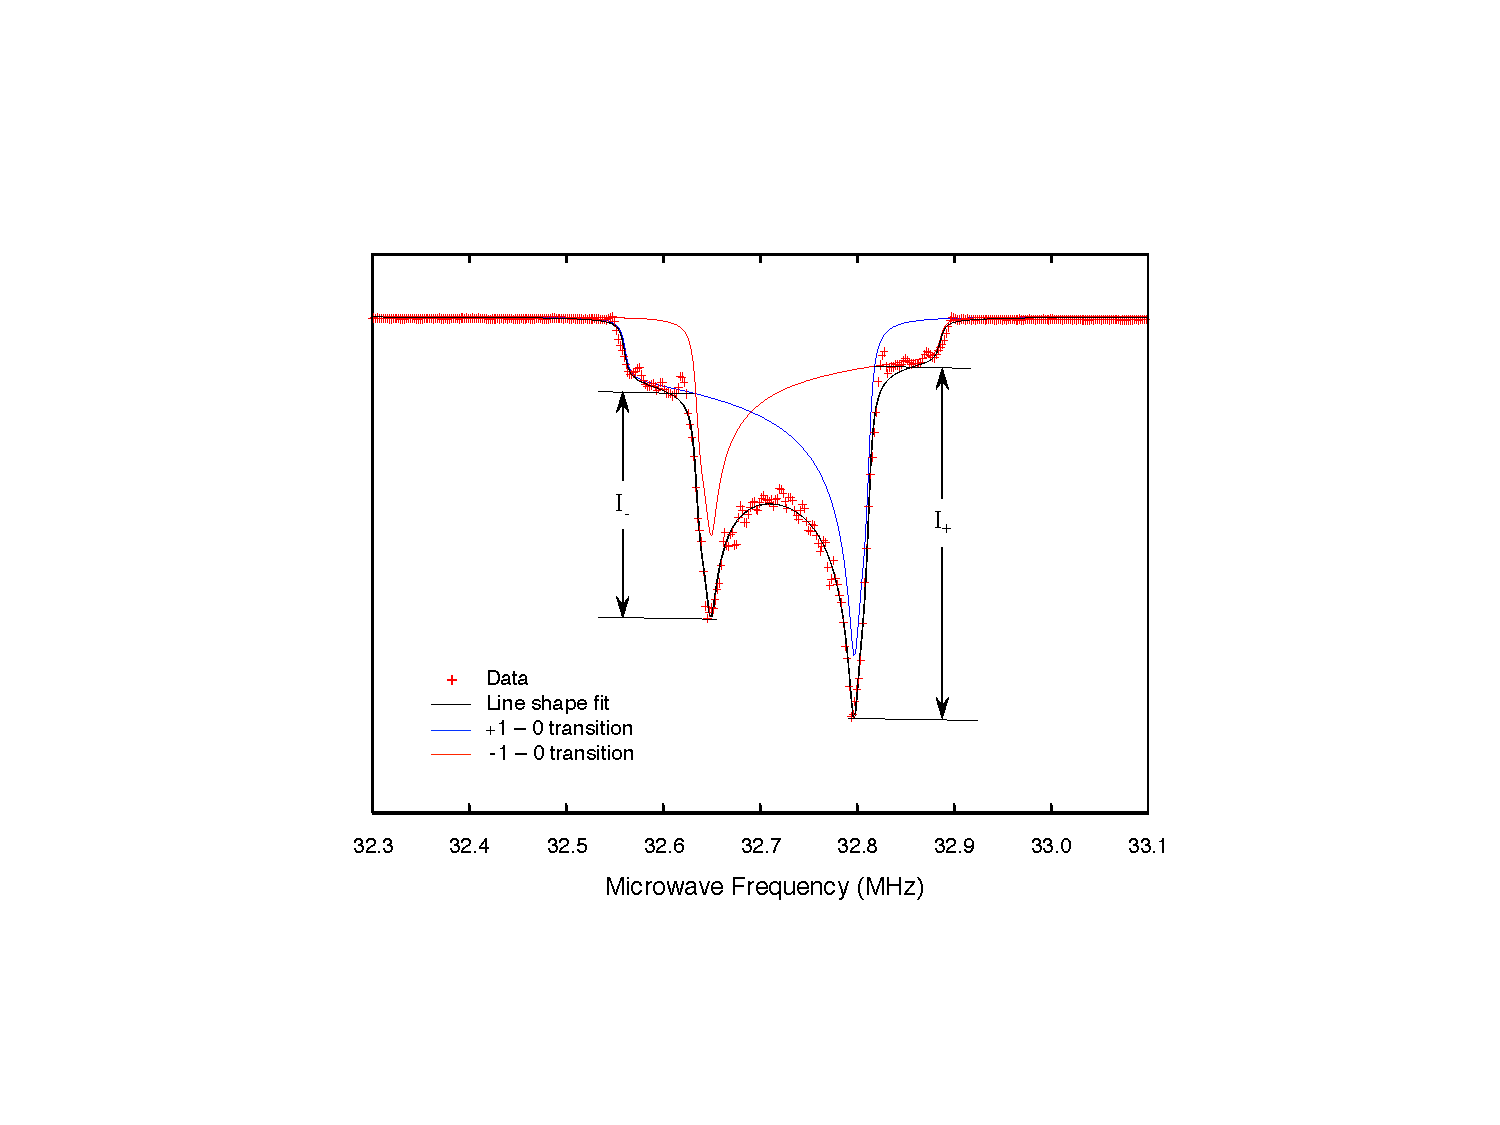
\includegraphics[width=3in]{Stache_NMR.pdf}
\end{center}
\caption{Typical NMR signal of polarized ND$_3$.  The black line results from a sophisticated line shape 
analysis of the data points and is a superposition of the two NMR transitions shown in red and blue.
This figure is adapted from~\cite{Kwaltine2013}.}
\label{NMR}
\end{figure}

\subsection{Luminosity}
The nominal length of the target container will be $L=4.0$~cm, and it will be filled with mm-sized granules of frozen $^{14}$ND$_3$ with a density $\rho =$ 1.007 g/cm$^3$ and a packing fraction $f\approx0.6$.  The total luminosity with electron beam current $I$ will be 
\begin{eqnarray}
	\mathcal{L}  & = & f \rho L N_A I   \\
& = & 0.6(1.007\, {\rm g/cm}^3)(4.0\,{\rm cm})(6.02\times10^{23}\,{\rm g}^{\minus 1})(6.24\times10^9\,{\rm s}^{-1}{\rm nA}^{\minus 1}) \nonumber \\
	                   & = & 9.1 \times 10^{33} \, {\rm cm}^{\minus 2} \,{\rm s}^{\minus 1} \,{\rm nA}^{\minus 1} \nonumber
\end{eqnarray}
Note that this number is per nA of incident beam current.  
The luminosity for scattering from polarized {\em neutrons\/} 
within the target will be $3/20$ of the above number, or 
$1.4 \times 10^{33}\,{\rm cm}^{\minus 2} \, {\rm s}^{\minus 1} \, {\rm nA}^{\minus 1}$.
We anticipate running the experiment at 10~nA, giving a neutron luminosity of $1.4\times10^{34} 
\,{\rm cm}^{\minus 2} \, {\rm s}^{\minus 1}$.



\section{Overhead for target operation}
There are four routine target operations that must be considered as overhead. 
First, we intend to provide an initial dose of approximately 20~Pe$^{\minus}$/cm$^2$ at 200~nA to each target sample prior to its use in the n-DVCS experiment.\footnote{1 Pe$^{\minus} = 10^{15}$ electrons.}  This is necessary to achieve the highest possible deuteron polarization, see below.  Second, the target must be periodically warmed to approximately 100~K in order to repair the deleterious effects of radiation damage, a process known as annealing.  Third, the target sample must be replaced when the anneals become ineffective at repairing the radiation damage.  Fourth, the NMR system will be periodically calibrated by performing
measurements of the thermal equilibrium polarization of deuterons at 5~T and temperatures around 1.4~K.
We examine each of this in the following sections, and a summary is made at the end.

\subsection{Cold dose}
In solid ammonia, paramagnetic radicals are created within the target sample by ionizing radiation, usually 
in the form of a 10--20~MeV electron beam, at a dose of about 
100~Pe$^{\minus}$/cm$^2$.
This is usually applied with the material cooled to 90~K with liquid argon, after which it may be stored indefinitely in liquid nitrogen.  The \.{N}H$_2$ (or \.{N}D$_2$) radical, which is stable to about 100~K (130~K), is understood to be responsible for the DNP process.  

In the case of {\em deuterated\/} ammonia, experience has shown that polarizations greater than 20\% are only achieved after an additional 
``cold'' dose of approximately 10~Pe$^{\minus}$/cm$^2$ has been applied to the sample at 1~K.  
The exact reason for this is not currently known.  One possible explanation is that at 1~K the electron beam 
creates additional paramagnetic species such as atomic deuterium that are not stable during the 90~K irradiation.  Their presence may alter the environment near the \.{N}D$_2$ radicals in some manner beneficial to DNP.  Whatever the reason, the effect can be dramatic.
During the EG4 program in Hall B, the deuteron polarization increased from an initial value under 20\% to more than 45\%  after a cold dose of  20~Pe$^{\minus}$/cm$^2$~\cite{Slifer2007}.  In this case, the CLAS detectors were turned off and a 100~nA beam was applied to the sample for an hour or so, followed by a 100~K anneal.  These cold irradiations were interspersed with normal data-taking at 2~nA, and the deuteron polarization was observed to increase after each anneal, eventually exceeding 45\%.  Rather than following this prescription, we intend to prepare each target sample with a 20~Pe$^{\minus}$/cm$^2$ cold dose before the experiment begins, using a single irradiation at 200~nA.  The CLAS12 detectors will be turned off for this procedure, which will require about a day for each sample. 

\subsection{Annealing}
As a solid polarized target material, deuterated ammonia has a remarkably high resistance to radiation damage, 
exceeded only by lithium hydride and lithium deuteride.
When exposed to ionizing radiation, the decay of the polarization is roughly exponential in manner,
\begin{equation}
	P = P_o e^{-D/\delta}.
\end{equation}
Here $D$ is the dose, measured in Pe$^{\minus}$/cm$^2$.
The critical dose $\delta$ of ND$_3$ is different for the positive and negative spin states, with
$\delta_{\plus} = 13$~Pe$^{\minus}$/cm$^2$ and $\delta_{\minus} = 26$~Pe$^{\minus}$/cm$^2$~\cite{Goertz2002}.  The polarization decay is due to the creation of additional paramagnetic species that do not contribute directly to the DNP process, but do contribute to the spin-lattice relaxation of the nuclear spins.
Fortunately, the concentration of these new radicals can be reduced by annealing the target sample at temperatures up to about 100~K for some tens of minutes.

For the purposes of this proposal, we assume an initial polarization of 45\%, which has been achieved 
in both the Hall C polarized target and the original Hall B polarized target.  To maintain an average polarization
of 40\%, the radiation damage must be repaired by annealing the target sample when the polarization falls to 35\%, or in other words, when the dose reaches 
$\minus \ln(\frac{0.35}{0.45})\delta \approx 5$~Pe$^{\minus}$/cm$^2$.  
Here we have used the average value of $\delta_{\plus}$ and $\delta_{\minus}$.  
Assuming a 10~nA beam current distributed evenly over a 2.4~cm diameter, 
this dose will be accumulated, on average, after 4 days.  We estimate a total of four hours will be required to anneal the target, cool it back to 1~K, and repolarize it to 40--45\%.

\subsection{Target lifetime}
During 80 days of beam time at 10~nA, the polarized target
will accumulate a total dose of 95~Pe$^-$/cm$^2$.
However, the maximum that a ND$3$ sample can tolerate before it must be replaced is not fully known.  
McKee~\cite{McKee2004} reports that for the Gen01 experiment in Hall C, a total of dose of
315~Pe$^{\minus}$/cm$^2$ was deposited on six different samples, and at least one continued to give high polarizations even after a dose of 100~Pe$^{\minus}$/cm$^2$.  The total dose had little or no effect on the frequency of anneals, although the maximum attainable polarization did decline slightly after about 
50~Pe$^{\minus}$/cm$^2$.   For this proposal we make the conservative estimate that the samples will be replaced after a total dose of 50~Pe$^{\minus}$/cm$^2$, of which 20~Pe$^{\minus}$/cm$^2$
will occur before data-taking begins.  The remainder will be incurred after about
25~days of data-taking at 10~nA, and so we anticipate that three samples of ND$_3$ will be sufficient 
for the entire experiment.  The time required to replace a sample, perform a TE calibration on the new sample, and to polarize it to 40--45\% should be about 8 hours.

\subsection{TE measurements}
Thermal equilibrium (TE) measurements are necessary to calibrate the NMR system,
and a TE must be performed whenever a new target sample is introduced into the experiment.  Additional
measurements are made throughout the experiment in order to monitor and reduce sources of systematic uncertainty such as gain drift and settling of the sample beads.   

To perform a TE, the target sample must first have its existing dynamic polarization destroyed, either by temporarily warming the sample or temporarily lowering the magnetic field to zero.  The sample must then be allowed to achieve its thermal equilibrium polarization, which it approaches in an exponential manner with a spin-lattice time constant $T_1$ that depends on the field strength, the sample's temperature, and its density of paramagnetic radicals. Since annealing the sample reduces its radical density and increases $T_1$, 
it is best to do TEs prior to the anneals.  Most measurements are made around 1.4~K, where the signal size is not too small, and $T_1$ is not too long.

Because the deuteron TE signal is small, a significant amount of signal averaging must be utilized to achieve a precise determination of its area, and so the time required for each measurement will depend strongly on the signal-to-noise ratio of NMR system.  Based on past experience, we assume four hours will be sufficient.  This includes the time required to polarize the sample to 40-45\% at the end of the calibration.

\subsection{Overhead summary}

\begin{figure}
\begin{center}
\includegraphics[width=5.4in]{Operation.pdf}
\end{center}
\caption{One possible sequence of target operations for the 80 day experiment. The numbers indicate the total dose accumulated during data taking, in Pe$^-$/cm$^2$. The experiment ends after 95~Pe$^-$/cm$^2$.
{\bf CD}: Cold Dose.  {\bf TE}: Thermal Equilibrium measurement.  {\bf A}: Anneal. }
\label{Operation}
\end{figure}
Based on the above information we provide the following estimate for the total overhead necessary to operate
the polarized target.  The total is 204 hours, or about 8 days.  Whenever possible, anneals and TE measurements can be coordinated with scheduled or unscheduled beam outages to lessen their impact on data acquisition.  One possible sequence is indicated in Fig.~\ref{Operation}.
\begin{enumerate}
	\item{Cold dose of 20~Pe$^{\minus}$/cm$^2$ at 200~nA.  Required: 3 @ 24 hours each.  \\
	Total: 72 hours.}  
	\item{Anneal every 5~Pe$^{\minus}$/cm$^2$.  Required: 17 @ 4 hours each.  \\
	Total: 68 hours.}
	\item{Change target sample after 30~Pe$^{\minus}$/cm$^2$.  Required: 2 @ 8 hours each.  \\
	Total: 16 hours.}
	\item{TE calibration of NMR system at the beginning of each target sample, and after 
	10~Pe$^{\minus}$/cm$^2$.  Required: 12 @ 4 hours each.  \\
	Total: 48 hours}.
\end{enumerate}




\bibliographystyle{model1a-num-names}
\bibliography{<your-bib-database>}
%% Authors are advised to submit their bibtex database files. They are
%% requested to list a bibtex style file in the manuscript if they do
%% not want to use model1a-num-names.bst.

%% References without bibTeX database:
\section{References}
\begin{thebibliography}{00}

\bibitem{Goertz2002} St. Goertz, W. Meyer, and G. Reichertz, Progress in Particle and Nuclear Physics {\bf 49} (2002) 403.

\bibitem{Slifer2007} K. Slifer, Proceedings of the 12th International Workshop on Polarized Ion Sources, Targets,
and Polarimetry, Upton, NY (2007) 330.

%\bibitem{Averett99} T.D. Avertt, et al., Nuclear Instruments and Methods in Physics Research Section A 427 (1999) 440. 

%\bibitem{Keith2003} C.D. Keith, et al., Nuclear Instruments and Methods in Physics Research Section A 501 (2003) 327.

%%\bibitem{Crabb97} D.G. Crabb and W. Meyer, Annu. Rev. Nucl. Part. Sci. 47 (1997) 67.

\bibitem{Court1993} G.R. Court, D.W. Gifford, P. Harrison, W.G. Heyes, and M.A. Houlden, 
Nuclear Instruments and Methods in Physics Research Section A 324 (1993) 433.

\bibitem{Court2004} G.R. Court, et al., 
Nuclear Instruments and Methods in Physics Research Section A 527 (2004) 253.

\bibitem{Dulya1997}  C. Dulya, {\em et.~al\/}, Nucl. Instr. and Meth. A \textbf{398} (1997) 109.

\bibitem{Kwaltine2013} N. D. Kwaltine, PhD thesis, University of Virginia, 2013.

\bibitem{McKee2004} P. McKee, Nucl. Instr. and Meth. A \textbf{526} (2004) 60.
\end{thebibliography}


\end{document}

%%
%% End of file `elsarticle-template-1a-num.tex'.
